\chapter{CN-VIP}\label{chap:cn-vip}

\margintoc{}

I already mentioned some of the typing rules related to memory actions and
pointer operations in \nameref{sec:kernel-mem-action-ops}, but I can now
recapitulate them with more detail, drawing special attention to parts about
liveness and bounds checks I omitted or skimmed past before. For convenience, I have
reproduced \cref{fig:typing-mem-action} in \cref{fig:cnvip-mem-action}.

Specifically, I will discuss the updated typing rules for memory actions and
pointer operations, and how I proved those typing rules sound with respect to
an updated model of \kl{ResCore} heaps. Lastly, I will explain how I proved the
\kl{ResCore} semantics as a sound abstraction above \kl{PNVI-ae-udi}.

\section{Memory actions}

\begin{figure*}[tp]
    \small
    \raggedright{}
    \onlyUseRules{\cndefnAction{}}{%
        \cndruleActionXXCreate{},
        \cndruleActionXXKillXXStatic{}
    }
    \onlyUseRules{\cndefnMemop{}}{%
        \cndruleMemopXXRelXXBinop{}
    }
    \caption{\kl{Kernel CN} typing rules for memory actions, and a select rule
        for typing a memory operation.}\label{fig:cnvip-mem-action}
\end{figure*}

In \textsc{Expl\_Is\_Action\_Create}, creating an allocation produces new
constraints on its base address and size. These are tracked via constraints on a
logical variable $\mathit{alloc}_\mathrm{var}$, a map from \kl{allocation ID}s to
pairs of a base address and size. This can be interpreted as an implicit
logical argument and return value for each function call.\sidenote{Need to
check the typing rules to ensure enforce this idea consistently.} Creating an
allocation also produces an \cninline{Alloc} token, to track the fact the
allocation is live, as well as the usual ownership/points-to resource.

TODO\@. Having a memory model also allows me to introduce support for dynamic
memory management. Whereas the above rule is only defined for typed objects
such as locals or globals, a region is essentially just an array of memory
bytes. For simplicity, I model every allocation as succeeding, so that the
pointer returned is never \cinline{NULL}. Hence the typing rule is similar,
but instead of ownership of a single object at a given C type, the ownership
is an iterated one over an array of memory bytes.

Conversely, in \textsc{Exp\_Is\_Action\_Kill\_Static}, destroying an allocation
requires both ownership of it (remember ownership represents read/write
permissions, but not allocation and freeing permissions), and the
\cninline{Alloc} token, plus proof that the given pointer is the same as the
owned pointer, and has the same base address as indicated by the allocation
token. For static kills (a block variable going out of scope), the rule also
checks that the size of the C type is also the size of the allocation.
TODO\@. Destroying a region is similar, except with an iterated ownership
of memory bytes.

Fortunately, the rules for loads and stores do not change at all. Ownership of
a location is enough to deduce that the allocation is live, and I assume
ownership is guaranteed to be in bounds for any allocation.\sidenote{Ownership
of out-of-bounds resources is equivalent to $\mathsf{false}$.}

\section{Pointer operations}

There are large discrepancies between the rules for pointer offsets presented
in \sidetextcite{lepigre2022vip} and \sidetextcite{memarian2022cerberus}, and
the \kl{Cerberus source code}, which I have detailed in a table in
\cref{fig:offset-confusion}. I am awaiting clarification on the correct way to
proceed.

\begin{figure*}[tpb]
  \begin{tabular}{ccccc}
  \toprule
   & \citeauthor{lepigre2022vip} incl.\ appendix & \citeauthor{memarian2022cerberus} & Cerberus code \\
  \midrule
  Member (P)
    & {\ballotX✗}
    & case \cinline{NULL}
    & case \cinline{NULL}, 0-offset
  \\
  Member (ISO)
    & bounds, case 0-offset
    & bounds, liveness
    & case \cinline{NULL}, 0-offset
  \\
  Array (P)
    & {\ballotX✗}
    & \textendash{}
    & \textendash{}
  \\
  Array (ISO)
    & bounds
    & bounds, liveness
    & bounds, liveness
  \\
  \bottomrule
  \end{tabular}
  \caption{Rules for computing pointer offsets (member and array, with
      pure/permissive (P) and ISO variants) in PNVI-ae-udi, across three
      different sources. `{\ballotX✗}' means the rule is omitted. `case'
      means the rule has a special case for that value. `\textendash{}' means
      there are no checks. `bounds' means a bounds check on the resulting
      pointer. `liveness' means a liveness check on the allocation.}\label{fig:offset-confusion}
\end{figure*}

Pointer operations such as taking the difference between two pointers or
relational comparison between two pointers, require both pointers to be in
bounds of the same live allocation. Hence the rule in\sidenote{TODO fix the
binop rule, which is a bit wrong in many ways} \cref{fig:cnvip-mem-action}
asks the solver to prove (a) the \kl{allocation ID}s are equal, (b) that the
pointer are within bounds of the allocation and (c) to check there exists a
live allocation with that ID\@. The evidence of a live allocation can be
either ownership with the same \kl{allocation ID}, or an \cninline{Alloc} token,
and the rule is agnostic as to which, just that this evidence is returned
in the type so as to not consume/destroy it.

A rule that is present in the code, but missing in other formats for
\kl{PNVI-ae-udi} is that for casting pointers to dead allocations to integers,
which is permitted so long as the address can fit within the target integer
type. Since \kl{VIP} does not track exposure, the live and the dead
pointer cases collapse into the same case. On top of this, as I mentioned in
\cref{subsec:prov-int-bytes}, I chose to support the limited provenance in
integers required via a new C type, to make any additional complexity and
performance cost as opt-in, and to avoid changing all the base types for
integers of various sizes (bit vectors) to a datatype with two constructors.
Because of these two simplifications, the cast is therefore just an identity,
on the SMT term and its base type.\sidenote{TODO add this rule} The rules for
casting an integer to a pointer is \kl{UB} if it is not in the \cinline{NULL}
or round-trip case, and is an identity in the latter.\sidenote{TODO add
this rule} And the rule for \cinline{copy_alloc_id} performs a bounds check on
the integer using the \kl{allocation ID} supplied by the pointer, and combines the
two into a new pointer.\cinline{TODO add this rule too}

The new C types need to be handled with care to implement the subtyping
required for a smoother experience.\sidenote{TODO figure out the subtyping
for base types and resources\ldots}

\section{\cinline{memcpy} and \cinline{memcmp}}

The typing rules for \cinline{memcpy} require iterated ownership of two
contiguous arrays of \kl{memory bytes} of length $n$; it returns ownership of
both, with the constraint that the value of the destination (first) is equal to
that of the source (second). The iterations must be contiguous and of the same
length to express the equality constraint on the values correctly.

The typing rules for \cinline{memcmp} require iterated ownership of two
contiguous arrays of \kl{memory bytes} of length $n$; like \cinline{memcpy}, it
returns ownership of both, unlike \cinline{memcpy} its resulting value is not
straightforward to specify, because the concise or obvious specification would
use quantifiers. I refer to a recursively defined logical function which
constrains the result to be (a) unconstrained if it reads any
\coreinline{unspec} values, (b) 0 if all bytes (excluding provenances) are equal
and (c) the difference between the first two unequal bytes otherwise. The presence
of \coreinline{unspec} values makes it difficult to give a simpler specification
to the result such as \cninline[breaklines]{src == dest && result == 0i3 || src
!= dest && result != 0i32}, because we do not wish to imply % chktex 26
\cninline{unspec == unspec}.\sidenote{The simpler specification could be
achieved with a notion of \emph{comparable bytes}, converting to which would
require ownership of only initialised and non-padding bytes.}

Both of these typing rules require a way to get ownership of memory bytes, for
which, \kl{CN-VIP} adds new annotations.\sidenote{TODO add these typing rules}
In the formal presentation, these are represented by operations on predicates
which consume ownership of an object, and produce ownership of memory bytes, or
vice versa.

\section{Soundness}\label{sec:cn-vip-soundness}

There are few steps involved to updating the formalisation to use a \kl{VIP}
based memory object model from its current concrete one.
\begin{enumerate}
    \item Extend the configuration of the dynamic semantics to be a step
        relation between abstract \emph{states} and expressions, rather than
        just \emph{heaps} and expressions.
    \item Extend the heap typing rules to incorporate the newly added
        allocation history.
    \item Update the proof of soundness for resource term reduction and pattern
        matching, with the new rules.
    \item Interpret and prove sound ResCore abstract state and transitions into
        the same for \kl{PNVI-ae-udi}, perhaps via an intermediate concrete
        memory model.
\end{enumerate}

\subsection{Extending the dynamic semantics}

In the typing rules, I modelled the allocation history as a single global
logical variable $\mathit{alloc}_\mathrm{var}$. This means that even morally
closed programs have that variable free in explicit logical and resource terms.
At the same time, because the allocation history is extended during the course
of evaluating a \kl{ResCore} program, it is not a term which can be substituted
once at the start of the program. Hence, the allocation history must
be threaded through to any part of dynamic semantics which relies on checking
constraints (in the empty context) using the SMT solver. At the point of
calling, the allocation history is substituted in, with the most up to date
information, to check the constraint as a closed term (\cref{fig:mem-model-dyn-smt}).

\begin{marginfigure}
    \small%
    \cndefnSubsXXSMT{}
    \caption{Calls to the SMT solver are now extended to thread through the
        changing allocation history.}\label{fig:mem-model-dyn-smt}
\end{marginfigure}

Only the \coreinline{create} memory action extends the allocation history, and
so it and every grammar node containing it also includes the allocation history
as part of its configuration, rather than threaded through the
side.\sidenote{TODO fix premise 7 of the create dynamic rules.} Note that
because I split the intuitionistic part of the allocation history from the
linear part, it does not get updated to record a dead allocation in the
rule for \coreinline{kill} (\cref{fig:mem-model-dyn-create-kill}).

\begin{figure*}
    \small%
    \raggedright%
    \begingroup%
    \NewCommandCopy{\origcndruleOpXXActionXXCreate}{\cndruleOpXXActionXXCreate}
    \renewcommand{\cndruleOpXXActionXXCreate}{\onlyUseNthCnPremise{1,2,3,7,8}{\origcndruleOpXXActionXXCreate{}}}
    \onlyUseRules{\cndefnOpXXAction{}}{%
        \cndruleOpXXActionXXCreate{},
        \cndruleOpXXActionXXKillXXStatic{}
    }
    \endgroup%
    \caption{The allocation history only tracks a mapping from IDs to a pair of
        base address and size, so when an allocation is killed, existing entries
        are not mutated.}\label{fig:mem-model-dyn-create-kill}
\end{figure*}

With the exception of threading through the allocation history, the rules for
loads and stores are unchanged. The rules for converting ownership of objects
into iterated ownership of memory bytes and vice versa are predicate
operations, much like the ones for manipulating structs and fixed-length
arrays.\sidenote{TODO add them} The rules for \coreinline{memcpy} and
\coreinline{memcmp} are also as expected.\sidenote{TODO add them}

Pointer operations do not extend the allocation history, but do require the
heap to check whether the supplied pointers belong to live allocations. They
are agnostic of whether it is ownership or an \cninline{Alloc} token is
provided as evidence (\cref{fig:mem-model-dyn-ptr-relop}).\sidenote{TODO
add/fix this}

\begin{figure*}
    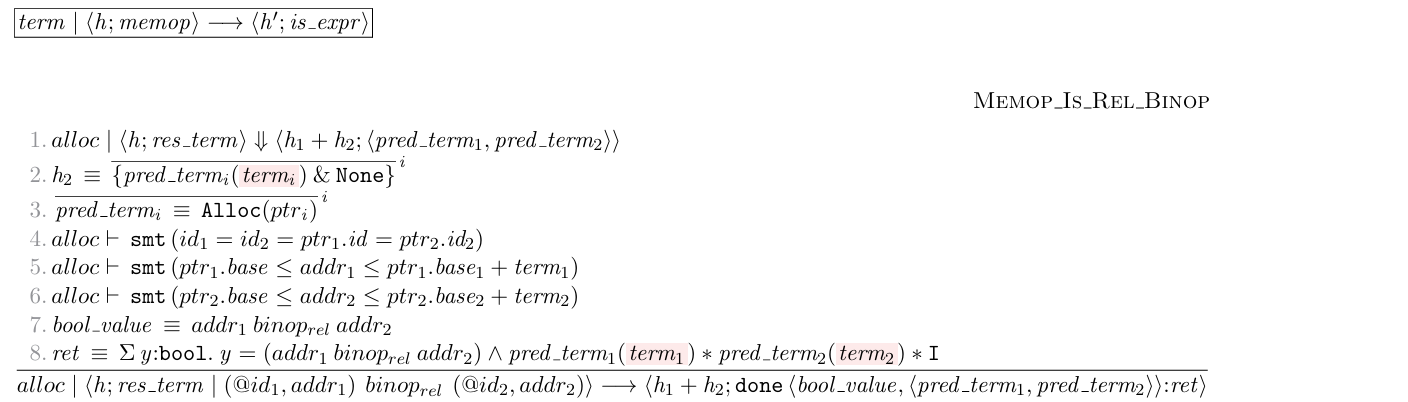
\includegraphics{figures/mem-model-dyn-ptr-relop}
    \caption{Memory operations involving pointers perform a bounds check using
        the SMT solver and supplied pointers, and a liveness check based on
        evidence from the supplied resource term and the heap.}\label{fig:mem-model-dyn-ptr-relop}
\end{figure*}

Lastly, there are the rules about pointer to integer casts, integer to pointer
casts and the \cinline{copy_alloc_id} primitive. The latter two check that that
resulting pointer is in the bounds of a live allocation; they are also agnostic
as to whether it is ownership or an \cninline{Alloc} token which is provided as
evidence.\sidenote{TODO this too\ldots}

\subsection{State typing}

Because the abstract state now includes an append-only allocation history, the
typing rules for heaps (\cref{sec:heap-types}) needs to be generalised to
include it. The main judgement involved in this is $\mathit{alloc} \Leftarrow
\Phi$, which says that the allocation history $\mathit{alloc}$ is consistent
with constraint context $\Phi$. \cref{fig:alloc-typing} shows that it does so
by checking if each constraint, with the allocation history substituted for the
$\mathit{alloc}_\mathrm{var}$, holds (under the empty context).

\begin{marginfigure}
    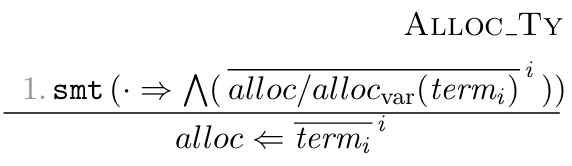
\includegraphics{figures/alloc-typing}
    \caption{Definition of a well-constrained allocation history \textemdash{}
        $\mathit{alloc}$ is consistent with each constraint in context
        $\Phi$.}\label{fig:alloc-typing}
\end{marginfigure}

The heap typing rule generalises similarly (\cref{fig:heap2-typing}). It
substitutes the allocation history for $\mathit{alloc}_\mathrm{var}$, and then
types the heap exactly as before.

\begin{marginfigure}
    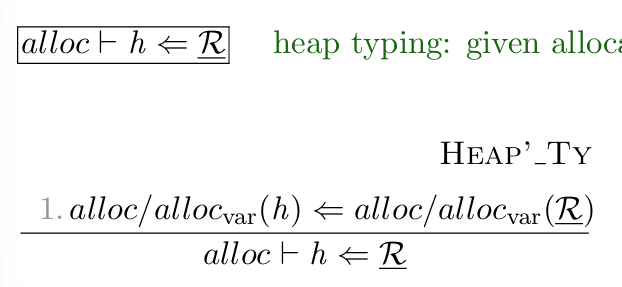
\includegraphics{figures/heap2-typing}
    \caption{Definition of heap typing in the presence of a allocation history:
        substitute the history into the heap and the type (\kl{normalised}
        resource context) and type as before.}\label{fig:heap2-typing}
\end{marginfigure}

\subsection{Updating the soundness proof}

Recall that I defined resource term reduction and pattern matching in the
dynamic semantics in a big-step style (\cref{sec:heap-types}). Whilst this
intertwines the proofs for progress and type preservation, its advantage of
modularity pays off now. The new constructs such as non-deterministic pointer
equality, \coreinline{allocate_region}, \coreinline{kill_dynamic},
\cinline{memcpy}, \cinline{memcmp}\cinline{copy_alloc_id}, and the conversions
to and from memory bytes, are just additional cases in the proof, the rest are
merely updates. The updates are small because the additional
constraints on the allocation history are easy to link across the static and
dynamic semantics by the definition of allocation history typing. The bounds
and liveness checks are similarly easy to link across the static and dynamic
semantics by the definition of heap typing. The updated theorem statements are
as below: the main differences are the use of the updated abstract state typing
judgements, and the use of the $\mathcal{L}_0 = {\; \mathit{alloc}_\mathrm{var}
\;}$ environment, instead of the empty one, for logical variables. Updated
proofs are in the appendix.

\begin{theorem}[CN-VIP:\ progress and type preservation for resource terms]
For all resource terms ($[[ res\_term ]]$) closed which type check or synthesise
($[[ cdot ; L0 ; N ; nR |- res\_term <= res ]]$), and well-typed states
($[[ alloct ; h <= N ; nR ]]$), there exists a resource value ($[[ res\_val ]]$),
context ($[[ nR' ]]$) and heap ($[[ h' ]]$), such that: the value is well-typed
($[[ cdot ; L0 ; N ; nR' |- res\_val <= res ]]$); the heap is well-typed
($[[ alloct |- h' <= nR' ]]$), and for all frame-heaps ($[[ f ]]$), the resource term
reduces to the resource value without affecting the frame-heap
($[[ alloct | < h + f ; res\_term > ||v < h' + f ; res\_val > ]]$).
\end{theorem}

\begin{theorem}[Progress for the annotated and let-normalised Core]
If a top-level expression ($[[ texpr ]]$) is well-typed
($[[ cdot ; L0 ; N ; nR |- texpr <= ret ]]$) and all computational patterns
in it are exhaustive, then either it is a value ($[[ tval ]]$), or it is
unreachable, or for all well-typed states ($[[ s <= N ; nR ]]$)
then there exists another state ($[[ s' ]]$) and expression ($[[ texpr' ]]$)
which is stepped to ($[[ < s ; texpr > --> < s' ; texpr' > ]]$)
in the operational semantics.
\end{theorem}

\begin{theorem}[Type preservation for the annotated and let-normalised Core]
For all closed and well-typed top-level expressions
($[[ cdot ; L0 ; N ; nR |- texpr <= ret ]]$),
well typed states ($[[ alloct ; h <= N ; nR ]]$),
frame-heaps ($[[ f ]]$),
new states ($[[ alloct' ; h' ]]$),
and new top-level expressions ($[[ texpr' ]]$),
which are connected by a step in the operational semantics
($[[ < alloct ; h + f ; texpr > -->  < alloct' ; heap ; texpr' > ]]$),
if all top-level functions are annotated correctly,
there exists a constraint context ($[[ N' ]]$),
sub-heap ($[[ h' ]]$),
and resource context ($[[ nR' ]]$),
such that the constraint context is extended
($[[ cdot ; L0 ; N ; cdot \sqsubseteq cdot ; L0 ; N' ; cdot ]]$),
the frame is unaffected ($[[ heap ]] = [[ h' + f ]]$),
the sub-state is well-typed ($[[ alloct' ; h' <= N' ; nR' ]]$),
and the top-level expression too
($[[ cdot ; L0 ; N' ; nR' |- texpr' <= ret ]]$).
\end{theorem}

\section{Linking \kl{ResCore} to \kl{PNVI-ae-udi}}\label{sec:linking}

\chapter{Implementation of CN-VIP}

\margintoc{}

In addition to designing, formalising, and proving it sound, I also implemented
CN-VIP\@. This was a substantial project which I worked on for about seven
months, from August to October of 2023, and May, June, September and October
of 2024.\sidenote{See
    \href{https://github.com/search?q=repo\%3Arems-project\%2Fcerberus+author\%3Adc-mak\&type=commits\&s=committer-date\&o=asc}{my commits}
    to the \kl{Cerberus} repository. In the intervening months, I
    worked on a failed update to the buddy allocator of pKVM to work with
    bitvectors (\cref{chap:buddy}), engineering for accurate source location
    information (\cref{sec:error-msgs}), and MiniCN (\cref{chap:kernel-alternative}).}

What made it more challenging was that it had to be developed and integrated
piecemeal alongside other active \kl{CN} development.

The first step was adding in the various pieces of infrastructure in a non-functional way.
\begin{itemize}
    \item A logical variable for allocation history.
    \item A resource predicate for the \cninline{Alloc} token.
    \item Updated rules for \coreinline{create} and \coreinline{kill}, using the \cninline{Alloc} token.
    \item A datatype for the SMT representation of pointers.
    \item A flag to toggle \kl{CN-VIP} features on and off.
    \item Array and member shifting operators.
    \item The \cinline{copy_alloc_id} operator.
\end{itemize}

Given all this, the next steps were about implementing support for bounds and
liveness checks, which was relatively straightforward.
\begin{itemize}
    \item Adapt and categorise the \kl{PNVI}/\kl{VIP} test suite to \kl{CN-VIP}\@.
    \item Support for non-deterministic pointer equality.
    \item Add a pointer liveness check.
    \item Deriving bounds and disjointness constrains.
    \item Basic support for \cinline{memcpy} (no provenance or
        \coreinline{unspec} values).
\end{itemize}

At this stage of development, I switched on CN-VIP by default, but retained the
ability to switch it off behind a flag. Fortunately, this happened just after
benchmarking on the CN tests was added, so we have a measurement of the impact
of the transition, shown in \cref{fig:vip-performance-hit}.

\begin{figure}[h]
    \centering
    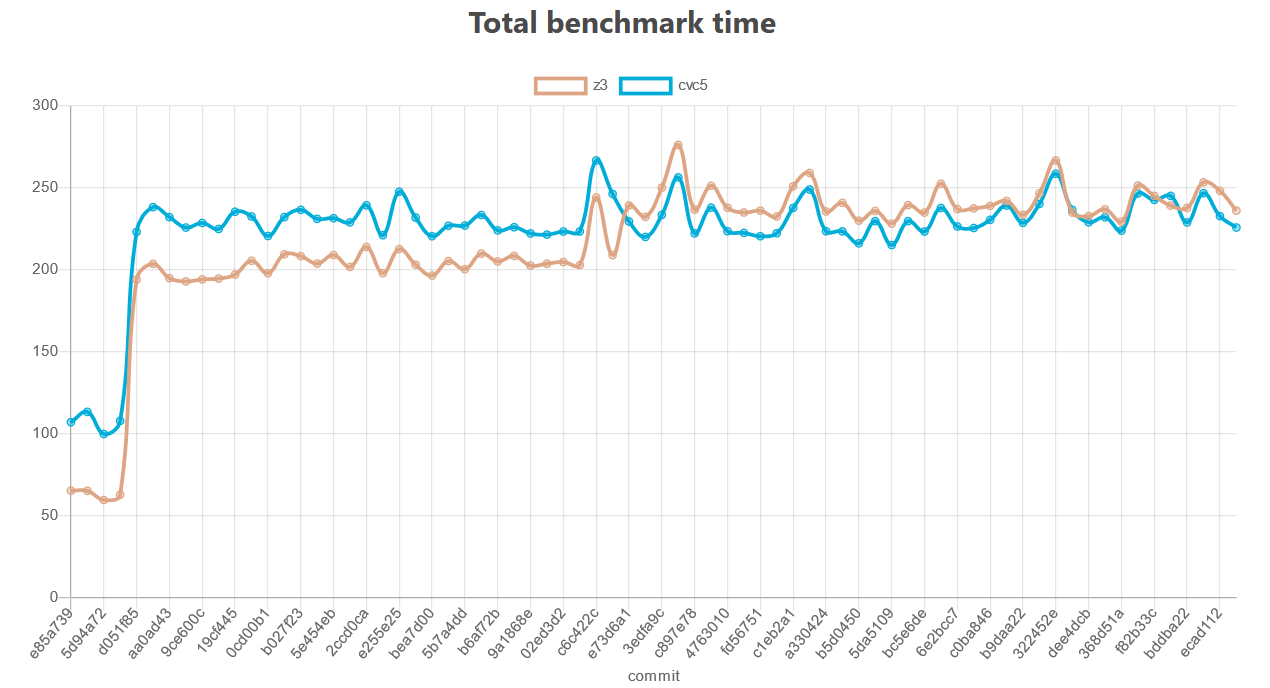
\includegraphics[width=\textwidth]{../misc/vip-performance-hit.png}
    \caption{Sharp increase in execution time when enabling VIP, courtesy of
        \url{https://rems-project.github.io/cn/dev/bench/}.}\label{fig:vip-performance-hit}
\end{figure}

Aside from performance, at this stage, it also became clear that not supporting
provenance in bytes was unworkable \textemdash{} 18 out of 44 tests required
additional \cinline{copy_alloc_id} annotations to work as intended. Lack of
support for round-trip was also an issue, this affected an additional 2 tests.

\begin{itemize}
    \item Support memory bytes.
    \item Support \cinline{memcpy}, \cinline{malloc} and \cinline{free}.
    \item Support comparable bytes for \cinline{memcmp}.
    \item Support round-trip casts.
\end{itemize}

\section{Definition of allocation history}

An allocation history is a map from \kl{allocation ID}s (non-empty provenances) to a
record of a base address and a size.

This is reflected in the definition of the \mintinline{ocaml}{Alloc.History}
module, below. Symbols are unique identifiers used to resolved names
immediately after parsing, whereas identifiers are wrappers around strings for
things like names of record fields. I omit the definition of the helper function
\mintinline{ocaml}{make_value} for space. Because I separate the intuitionistic
and linear facts about the allocation history, this is all that is required to
declare it.

\ocamlfile{code/alloc_history.ml}

This is brought into the `empty' typing context, so that it is always in scope
for checking any function, which simply adds the symbol, its type, and some
location information (a built-in variable). Notably, there are no constraints
on it at the beginning.

\ocamlfile{code/empty_context.ml}

\section{Definition of \cninline{Alloc} token}

A definition of a predicate is a record of a location, a symbol for the first
pointer argument, a list of any other input arguments, a type for the output
argument, and an optional list of clauses (the body, potentially guarded by a
series of top-level ifs). The clauses represent the contents of the predicate,
if it can be unfolded (\cninline{Owned} and \cninline{Block} are built-in and
so cannot be unfolded).

\ocamlfile{code/definition_predicate.ml}

Using this, an \cninline{Alloc} token is defined simply as a predicate which
takes only the special pointer argument, no other input arguments, outputs the
record of base address and size, and has no clauses, i.e.\ cannot be unfolded.

\ocamlfile{code/definition_alloc.ml}

This is registered in an environment of definitions and declarations, in the
\ocamlinline{Global} module. Unlike the previous environment, this one does not
change during the course of type checking, but is populated on a per-file
basis. The symbol for \cninline{Alloc} tokens is mapped to the definition
mentioned earlier.

\ocamlfile{code/global_alloc.ml}

The Cerberus front-end supports an extension point, so that the
\cninline{Alloc} token, the \cninline{allocs} logical variables, and other
built-in symbols can be resolved correctly.

\section{Using \cninline{Alloc} in \coreinline{create} and \coreinline{kill}}

These constructs are introduced either by the user, or by a \coreinline{create}
action. Whilst in the formalisation the rules for memory actions are very
clearly synthesising, in the implementation they are more mixed, where terms
are synthesised, but base types are checked, and the contexts are changed along
the way.

The \coreinline{create} action takes as its arguments a pure expression for expressing
the alignment of the new allocation \ocamlinline{pe}, a C type \ocamlinline{act} and some
source location information \ocamlinline{prefix}. The latter is used only to generate
a helpful name for the logical variable representing the returned pointer.

First the base types are checked to line up, and then the alignment expression.
The continuation for checking the alignment expression names the result as
\ocamlinline{arg}, which is used to create the alignment value
\ocamlinline{align_v}. The return value \ocamlinline{ret} is defined, and a
fresh symbol is created \ocamlinline{ret_s} and added to a (unified) variable
context using \ocamlinline{add_a}. The function \ocamlinline{add_c} adds the
constraint that the return value \ocamlinline{ret} is aligned to
\ocamlinline{align_v} to the constraint context. Similarly, \ocamlinline{add_r}
adds the uninitialised ownership resource to the resource context.

\ocamlfile[lastline=18]{code/check_create.ml}

After that, the VIP related code begins. To express bounds constraints on the
new allocation, a constraint that the value keyed by the pointer (actually its
provenance) in the allocation history will equal a record of the return address
and C type size. Note that this constraint is added under a flag
\ocamlinline{use_vip} (the `!' in OCaml is for reading a (mutable) reference,
not for negation). The allocation token is added immediately afterwards. The
typing context logs this action for error reporting, and then passes the
resulting value to an explicit continuation \ocamlinline{k}.

\ocamlfile[firstline=19]{code/check_create.ml}

\section{SMT representation of pointers}

Allocation IDs (non-empty provenances) have their SMT representation
switchable. If VIP is enabled, the representation is just an integer, otherwise
it is the empty tuple.

\ocamlfile[lastline=4]{code/solver_pointer.ml}

Pointers build on this switchable representation, so do not need a switch
themselves. Their SMT representation is a datatype named
\ocamlinline{"pointer"}, which is not polymorphic \ocamlinline{[]}, with two % chktex 18
constructors \ocamlinline{NULL} (which takes no arguments) and
\ocamlinline{AiA} for `\kl{allocation ID} and address' which takes two arguments,
\ocamlinline{"alloc_id"} of type \ocamlinline{CN_Alloc_Id.t ()} and % chktex 18
\ocamlinline{"addr"} of type bit vector (of a width determined by the memory % chktex 18
interface).

\ocamlfile[firstline=20]{code/solver_pointer.ml}

\section{Array and member shifting}

I will only show the code for member shifting; the code for array shifting is
very similar.

Bounds check constraints are as expected \textemdash{} a lookup in the
allocation history followed by constraints that the address of the pointer
(assumed to have an \kl{allocation ID}) must be between the base and base plus
size.

\ocamlfile[lastline=8]{code/check_member_shift.ml}

Having created the constraints, the check for the bound and liveness are gated
by the flag to enable VIP or not. First, it checks the allocation is live.
Next, if the SMT solver can prove the bounds check statically, based on the
available constraints, it will quietly succeed; if not, it will raise an error
saying the allocation for \ocamlinline{term}, is out of bounds
(\ocamlinline{constr} could not be proven), resulting in the \kl{UB} specified
by \ocamlinline{ub}, with \ocamlinline{model} as the counter-example.

\ocamlfile[firstline=10,lastline=24]{code/check_member_shift.ml}

The member shift constructor takes as its arguments a \ocamlinline{pe}
representing the struct address to shift, the struct type \ocamlinline{tag},
and the field \ocamlinline{member}. After the base types are checked, and
\ocamlinline{pe} has been type checked and symbolically evaluated to
\ocamlinline{vt} (value term), first it is checked to have an \kl{allocation ID}
(not be \cinline{NULL}), and then (assuming strict pointer arithmetic) checked to
be in bounds of a live allocation.\sidenote{As explained in the comment in the
code, this check is technically redundant because the elaboration guarantees
that every use of \coreinline{member_shift} is preceded by a call to
\coreinline{PtrValidForDeref}, which checks that the pointer is live and
strictly within bounds (not one past). However, since relying on this is a bit
fragile, I implement the checks anyway.}

\ocamlfile[firstline=26]{code/check_member_shift.ml}

\section{Adding copy\_alloc\_id}

Checking \cinline{copy_alloc_id} has a similar pattern. It checks the base
types, and checks and symbolically evaluates the two arguments. After it does so,
it checks the pointer is not \cinline{NULL}, and then checks the resulting
pointer is in bounds of a live allocation.

\ocamlfile{code/check_copy_alloc_id.ml}

\section{Adapting the PNVI/VIP test suite for CN}

I had to adapt the PNVI/VIP test suite to run with CN in a few ways. First,
because \kl{CN} does not (yet) support \cinline{printf}, I replaced the print
statement with assertions about the expected values at that point in the
program.

Secondly, some of the tests were intended to trigger the non-deterministic
pointer equality. It is not possible to write an assertion that a value
is \emph{not} constrained, and so for that, I used macros
(\cinline{NON_DET_TRUE} and \cinline{NON_DET_FALSE}) as a switch. I show the
example from \cref{fig:nd-ptr-eq-example}, adapted to test CN VIP, below.

\cfile[fontsize=\footnotesize,breaklines]{code/provenance_equality_global_yx.nondet.c}

In addition to checking a variable is \emph{not} constrained, I also needed to
check that some tests fail without \cinline{copy_alloc_id} annotations, and
pass with them. An example of this below, is using exclusive-or to manipulate
and reconstruct and valid pointer address via an integer. Under VIP, the only
way to recover its provenance is to use \cinline{copy_alloc_id}, so the test
must be run both ways to ensure it errors and succeeds appropriately.

\cfile[fontsize=\footnotesize,breaklines]{code/pointer_offset_xor_auto.annot.c}

Finally there are tests which should just pass with no annotations, which I
omit for space.

\section{Non-deterministic pointer equality}

I implement pointer equality and pointer inequality using the same function and
a flag for when the differences arise. In particular, after the base types are
checked, the continuation is re-bound to take the negation of the value at the
end in the negated case.

\ocamlfile[lastline=5]{code/check_ptreq.ml}

After the two operands are checked and symbolically evaluated to
\ocamlinline{arg1} and \ocamlinline{arg2}, I define a helper function to create,
constrain and return a variable.

\ocamlfile[firstline=6,lastline=13]{code/check_ptreq.ml}

I then define the circumstances under which the result is ambiguous: when both
pointers have \kl{allocation ID}s, differing provenances but equal addresses.

\ocamlfile[firstline=14,lastline=27]{code/check_ptreq.ml}

If the solver cannot statically rule out the ambiguous case, a warning is
issued to the user.

\ocamlfile[firstline=28,lastline=41]{code/check_ptreq.ml}

The true case, when both pointers are equal, is easy to define as a constraint.

\ocamlfile[firstline=42,lastline=44]{code/check_ptreq.ml}

The false case, is defined by negation \textemdash{} neither the both-equal
case, nor the ambiguous case.

\ocamlfile[firstline=45,lastline=49]{code/check_ptreq.ml}

Unlike other rules, the result in this case is not a value, a boolean variable
which is constrained to be true in the both-equal case, and to be false in the
neither-equal-nor-ambiguous case. I do not need to state the contrapositive
implications since SMT solvers assume classical logic. The ambiguous case
leaves the result under-determined by omission, and the result is passed to the
continuation.

\ocamlfile[firstline=50]{code/check_ptreq.ml}

\section{Checking whether a pointer is live}

A check for a live allocation can end in finding a live resource, not finding
one because the resource context has no ownership or allocation tokens, and not
finding one because there was no match (thus resulting in a counter-example).

\ocamlfile[lastline=8]{code/inference_liveness.ml}

Given a resource, an accumulator \ocamlinline{found}, and a candidate pointer
with an \kl{allocation ID} \ocamlinline{res_ptr}, if an answer has already been
found, then skip past this resource, otherwise check if the solver can
statically prove the searched pointer \ocamlinline{ptr} and it have the same
\kl{allocation ID}\@. If that is the case, then signal a resource has been found,
otherwise save the counter-example from the failed proof attempt.

\ocamlfile[firstline=9,lastline=22]{code/inference_liveness.ml}

Given a resource, and an accumulator \ocamlinline{found}, if the resource is
ownership or an allocation token, then check use the pointer from that resource
as a candidate for checking whether it and the search pointer have equal
\kl{allocation ID}s.

\ocamlfile[firstline=23,lastline=36]{code/inference_liveness.ml}

This function is folded over the entire resource context, and missing live
allocations are signalled as errors, with or without the most recent
counter-example.

\ocamlfile[firstline=37]{code/inference_liveness.ml}

\section{Deriving disjointness and bounds constraints on pointers}

One unexpectedly inconvenient aspect of pointers which are partly concrete is
that disjointness facts are expressed over intervals rather than points. This
means that the `distinct' operator provided by some SMT solvers is not
useful.

Instead, such facts must be derived from the resource context. For
example, for a single ownership in the context, we may deduce that (a) it has
an \kl{allocation ID} (is not \cinline{NULL}), that the range of addresses it
owns does not wrap-around (the base is less than its upper bound), and that, (b) if
\kl{VIP} is enabled, there exists an allocation which contains it.

\ocamlfile[lastline=15]{code/resource_derived_lc.ml}

Similarly, if \kl{VIP} is enabled and an \cninline{Alloc} token is in the
resource context, we may deduce the intuitionistic constraints associated with
it: the output argument of that resource is the same as the lookup in the
\cninline{allocs} allocation history keyed by the allocation ID of its pointer,
and that the allocation does not wrap-around. Other constraints, including iterated
constraints, do not have any constraints derived from them \textemdash{} this is
likely to need to
change.\sidenote{\url{https://github.com/rems-project/cerberus/issues/541}
    shows that users would like to have disjointness information inferred from
    iterated ownership.}

\ocamlfile[firstline=16,lastline=23]{code/resource_derived_lc.ml}

Constraints may also be derived from pairs of resources in the context, such as
the fact that simultaneous ownership implies the range of owned addresses are
disjoint.\sidenote{This is one of the few places in \kl{CN} that disjunctions
constraints are added to the context.}

\ocamlfile[firstline=25,lastline=35]{code/resource_derived_lc.ml}

Deriving constraints is necessary for soundness but incurs a non-trivial
performance penalty. Hence, there is a flag for disabling it (experimental).
Care must also be taken to not re-derive the same facts, since this also seems
to result in a performance hit to the SMT
solver.\sidenote{\url{https://github.com/rems-project/cerberus/pull/436}}

\ocamlfile[firstline=37]{code/resource_derived_lc.ml}

The facts are derived every time a new resource is added to the context.
They are added to the constraint context because they need to persist,
even if the resource is consumed (for example, consuming ownership
of two pointers does not change the fact that they were and still
are unequal).

\ocamlfile{code/typing_add_r_internal.ml}

\section{Basic support for \cinline{memcpy}}

To understand the impact and importance of having provenance in
bytes, I initially specified \cinline{memcpy} merely to copy iterated
ownership of characters. I derived the initial version of the specification
from verifying a user-defined version of \cinline{memcpy}, which copied an
array character by character. The specification ends with a quantified constraint,
saying the arrays are equal over the given range. This is because the SMT arrays
are total (not finite), and stating a constraint which says the arrays are equal
would spuriously fail with a counter-example index outside of the intended range.

\cfile[fontsize=\footnotesize,breaklines,firstline=9,lastline=23]{code/pointer_copy_user_dataflow_direct_bytewise.c}

To use this in the intended way, one has to use a lemma that the terms are
equal at all indices. The proof of the lemma in Rocq would rely on the fact
that the terms are defined with respect to iterated resources which cover the
same finite range.

\begin{figure}[h]
\cfile[fontsize=\footnotesize,breaklines]{code/cn_lemmas_byte_arrays_equal.h}
\caption{\kl{CN} lemma that two ``byte'' (\cinline{unsigned char}) arrays
    are equal if they have the same elements over a finite range. This needs
    to be a lemma because of the mismatch between the intended finite nature
    of arrays and the total nature of the ones use by SMT solver.}\label{fig:byte-array-eq-lemma}
\end{figure}

However, when typing a built-in, I can simply combine the two so that users do
not need to use lemmas after calling \cinline{memcpy}.

Though there is nothing in principle which forces the specification of
\cinline{memcpy} to be one that is expressible in the surface syntax (for
example, the specification simply skipped over the byte representation and
copied resources in a polymorphic way), there are practical limitations.

The issue stems from the fact that calls to \cinline{memcpy} are
replaced with calls to a proxy \kl{Core} procedure during \kl{Cerberus}'
elaboration. The proxy procedure wraps up a call to the memory interface
operation for coreinline{memcpy}. During type checking, \kl{CN} only
sees the call to the proxy, and not the memory operation. There is no
convenient way to inline the body of the procedure, so the next best
option is to give it a type like every other function and built-in
procedure.

\section{Insufficiency of not tracking provenance in bytes or integers}

The lack of provenance in bytes presents a major limitation to expressiveness
of the memory object model. Consider the below call to the
\cinline{user_memcpy} specified before (the same issue arises with the built-in
\cinline{memcpy}, sans the application of the \cinline{byte_arrays_equal}
lemma).

\cfile[fontsize=\footnotesize,breaklines,firstline=48]{code/pointer_copy_user_dataflow_direct_bytewise.c}

The issue is that upon converting ownership of pointers \cinline{&p} and
\cinline{&q} into bytes, the type system loses the provenance they carry. And
hence, when those bytes are converted back into pointers, they have an
$@\mathsf{empty}$ provenance.

A temporary work-around for this is to \cinline{copy_alloc_id} the
provenance back, but this just happens to work because the original pointer is
in scope. If it was not, then the example could not be rescued. And as it
happens, the lack of provenances in bytes affects 18 out of 44 tests, and a
lack of provenance in integers affects another 2.


\section{Memory bytes and their use in \coreinline{memcpy}, \coreinline{malloc}
and \coreinline{free}}\label{sec:mem-bytes-use}

\section{Comparable bytes in \coreinline{memcmp}}

\section{Integer with/out provenance union type for round-trip casts}

\chapter{Epilogue on CN-VIP}

Having finished my discussion on the formalisation and implementation of
\kl{CN-VIP}, I will now discuss the aftermath of transitioning the \kl{CN} test
and tutorial code to using it. I will finish with a discussion on how future
work could use the principles uncovered by my work to place the \kl{CN} memory
model on more foundational and trustworthy footing.

\section{Performance}\label{sec:vip-perf}

\kl{CN-VIP} causes a significant hit to performance. The benchmarks below show
a 2\textendash{}3x slowdown, though this is imperfect because some tests are intended to
fail in early stages such as parsing, desugaring or well-formedness checks.

\begin{figure}[h]
    \centering
    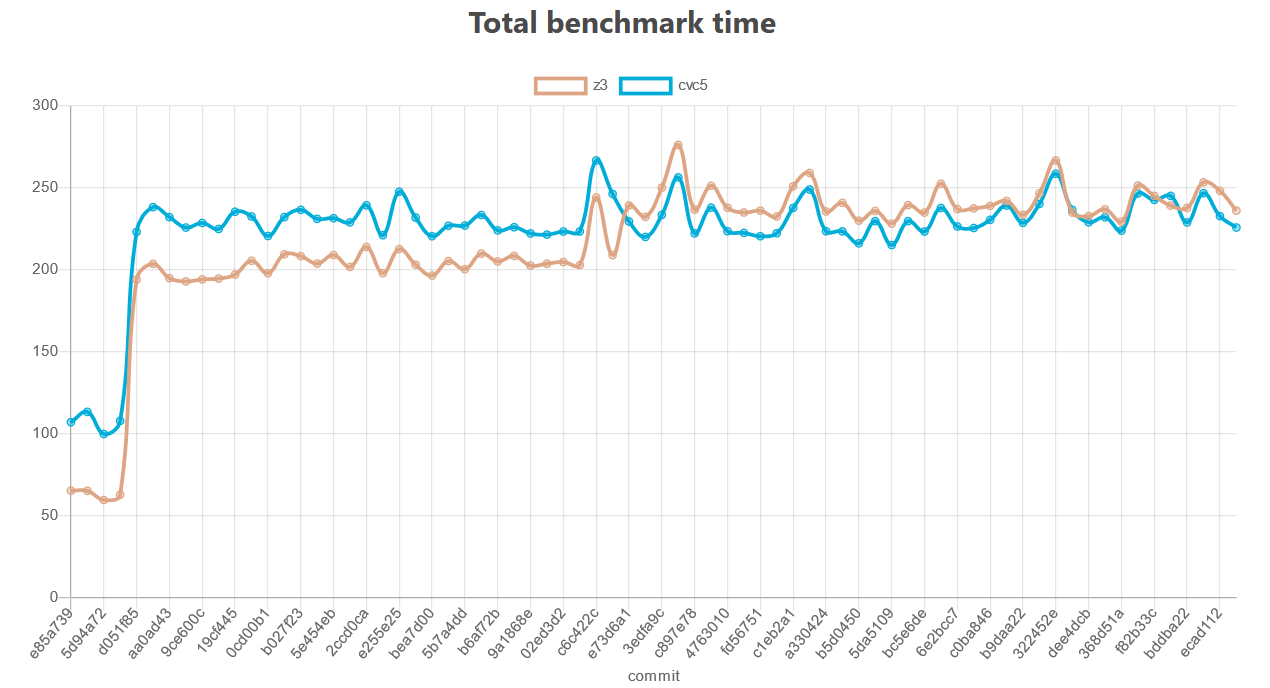
\includegraphics[width=\textwidth]{../misc/vip-performance-hit.png}
    \caption{Sharp increase in execution time when enabling VIP, courtesy of
        \url{https://rems-project.github.io/cerberus/dev/bench/}.}\label{fig:vip-performance-hit2}
\end{figure}

% It is more fruitful to look at the tests individually, and see which ones
% show a demonstrable slowdown when \kl{VIP} was enabled.
%
% \begin{itemize}
%     \item block\_type.c (CVC5, 4x)
%     \item implies2.error.c (CVC5, 2x)
%     \item extract\_verbose.c (CVC5, 5x)
%     \item builtin\_ctz.c (CVC5, <2x)
%     \item disj\_nonnull.c (both, <2x)
%     \item gnu\_types\_compatible.c (CVC, <2x)
%     \item tree16/as\_partial\_map/tree16.c (both, 3/4x)
%     \item tree16/as\_mutual\_map/tree16.c (both, 3x)
%     \item fun\_ptr\_extern.c (CVC5, 4x)
%     \item increments.c (both, 10x)
%     \item has\_alloc\_id\_shift.c (both, <2x)
%     \item int\_to\_ptr.c (both, <2x)
%     \item has\_alloc\_id\_ptr\_neq.c (both, <2x)
%     \item fun\_ptr\_three\_opts.c (Z3 <2x, CVC5 4x)
%     \item has\_alloc\_id\_ptr\_eq.error.c (CVC5 2x)
%     \item ptr\_diff2.error.c (both <2x)
%     \item ptr\_relop.error.c (both 2/3x)
%     \item ptr\_diff.errro.c (Z3 <2x, CVC5 3x)
%     \item bitwise\_compl.c (CVC5 2x)
%     \item alloc\_token.c (both <2x)
%     \item implies\_precedence.c (CVC5 2x)
%     \item division\_casting.c (Z3 <2x, CVC5 2x)
%     \item reverse.c (Z3 6x, CVC5 5x)
%     \item mask\_ptr.c (Z3 <2x, CVC5 3x)
%     \item and\_or\_precedence.error.c (CVC5 <2x)
%     \item get\_from\_arr.c (Z3 2x, CVC5 3x)
%     \item enum\_and\_and.c (both 2x)
%     \item simplify\_array\_shift.c (CVC5 5x, Z3 7x)
% \end{itemize}

% There are three potential reasons for this.
% \begin{enumerate}
%     \item Pointer bounds checks.
%     \item Pointer liveness checks.
%     \item Deriving constraints.
% \end{enumerate}

There are two main components to \kl{CN-VIP}: the pointer liveness checks, and
the bounds checks. Disabling the liveness checks is simple and gives sensible
timing information: tests which passed before will continue to do so; tests
which failed because pointers could not be proved live are small ones which do
not test anything afterwards. Disabling liveness has barely any impact on the
total time taken (a slight increase, because of previously failing tests now
passing) and so what remains is the bounds checks.

The bounds checks are easy to disable, but this does not lead to a fair
comparison: of course we expect the version which checks less and unsoundly to
go faster. Furthermore, any slow down for bounds checks will be some mixture of
the effect of derived constraints, and the complexity of the check itself.

The above two facts combined\sidenote{And a few hours of experimentation}
suggest a possible remedy: if any bounds checks can be replaced with checks in
the resource context, then it may offer a substantial speed-up. Since ownership
of a pointer is sufficient (but not necessary) to deduce bounds checks, we can
replace some of those with checking the resource context for ownership.

In particular, for member and array shifts, this is a good strategy, because
often the shifting is done just before loading, for which ownership needs to be
present regardless. The ownership check can be done first, and if it fails, the
code will fall back to the slower, full check.

The net result of this is a substantial speed-up of CN-VIP overall: a 3x
slowdown is now less than 50\% slowdown, which although not ideal, is a
worthwhile improvement. Although \kl{VIP} increases complexity and slows
things down considerably, it did also provide a helpful equivalence which I
exploited to improve execution time.

However this does raise questions: why is a linear lookup in the resource
context faster than proving a pure SMT constraint? One possibility is that most
equalities tested in resource lookup can be resolved syntactically without
appeal to the solver. This may just be an empirical fact about most C programs,
and although not very theoretically elegant, still useful. Another possibility
is that the encoding of the allocation history bounds constraints is
sub-optimal. TODO discuss with CVC5 folks.

It is possible to optimise further, for example, the \kl{Core} elaboration
performs a \coreinline{PtrValidForDeref} check before every
\coreinline{member_shift}, and so the checks on the \coreinline{member_shift}
itself are technically redundant. Though perhaps a bit fragile, such facts
could be exploited (maybe behind a switch) to improve performance of
\kl{CN-VIP} even more.

\section{Updating existing code}

As I was developing \kl{CN-VIP}, I was testing it under a flag, adding new
tests and updating existing ones. Generally, \kl{CN-VIP} is more strict than
the previous model, and so it was easy to update tests in a
backwards-compatible manner. Where VIP added new expressiveness, I added new
tests, separate from the existing regression suite. Importantly, the new ones
included a mix of positive and negative tests.

This makes it more difficult to quantify the impact of \kl{CN-VIP} on existing
code. However, unlike the regression suite, I left the \kl{CN tutorial}
examples until implementation was stable, and out of fear that I would have to
spend weeks updating more than two hundred small tests to handle the stricter
rules.

Thankfully, my fears turned out to be unnecessary, as
\href{https://github.com/rems-project/cn-tutorial/commit/9ee153e74d1b0fbdcb2802f2186d211ab6b2343b}{commit
9ee153e7}, `Add support for VIP', demonstrates. Out of roughly 185 small,
``working'' test cases, only 7 had to be updated.\sidenote{A limitation of the
    testing framework for the tutorial, and at the time, the \kl{CN} regression
    suite, is that it only checks returns codes, not the whole output. So there
    was no automated way of checking whether an already failing test starts
failing for a different reason. I eventually fixed this
\href{https://github.com/rems-project/cerberus/pull/703}{(cerberus/\#703)} by
capturing all output and automatically diffing it.} Four of them were
related to casting integers to pointers, of which one was a round-trip which
was not supported initially. All of them were updated using
\cinline{copy_alloc_id}.

\inputminted[fontsize=\footnotesize,breaklines,firstline=10,lastline=68]{diff}{code/add_support_for_vip.patch}

\subsection{Catching \kl{UB}, as intended}

The other three were all related to \emph{decrementing} a pointer out of
bounds, and technically \kl{UB}, and so assuming the intent was to test pointer
decrementing rather than catching \kl{UB}, I adjusted the code to either not
decrement the pointer, or increase the size of the allocations involved to allow it.

\inputminted[fontsize=\footnotesize,breaklines,firstline=69,lastline=107]{diff}{code/add_support_for_vip.patch}

\subsection{Non-deterministic pointer equality}

The other set of examples were the approximately 81 C files (114 including
headers) used in the \kl{CN tutorial}. Of these, 7 were intentionally broken in
non-\kl{VIP} ways for pedagogical reasons, which I manually checked was
preserved after the transition. Another 4 were intentionally without
annotations, of which 3 started to fail verification earlier because of
\kl{VIP} related reasons (member shifting on a pointer not guaranteed to be
non-\cinline{NULL}). Of the remaining 70 C files (103 including headers), only
2 predicate definitions (in headers) and 2 lemmas needed updating. The latter
followed from the former because the lemmas simply inlined the definitions of
the predicates.

\inputminted[fontsize=\footnotesize,breaklines,firstline=108]{diff}{code/add_support_for_vip.patch}

As one can see, all the updates were related to excluding the non-deterministic
case in pointer equality in a queue example.\sidenote{A detailed walk-through
is available online:
\url{https://rems-project.github.io/cn-tutorial/getting-started/case-studies/imperative-queues/}.}
Specifically, because the implementation for the pop operation, and the C proof
of an induction lemma to verify the push operation, both used C's pointer
equality, the predicates for that datatype needed an additional constraint that
address equality implied pointer equality for the relevant pointers. This is
enough to assuage \kl{CN-VIP} that the non-deterministic pointer equality case
is impossible. The constraint is sensible and the example still usable because
the pointers refer to a node in a queue; thus, they need to be valid for
dereferencing (not one-past), hence ruling out the possibility that they could
have equal addresses and differing provenances.

\section{Lemma proofs within C}\label{sec:lemma-proof-c}

As visible above, the queue example requires the use of lemmas to prove the
appropriate facts for popping and pushing. I did not write the implementation
for these examples, but I did verify them completely, including proofs of
lemmas using C as a tactic language.

The experience was humbling because I found it quite difficult; it took a few
days work. This was mostly due to my lack of prior experience with separation
logic proofs about basic data-structures such as linked list, and resulting
lack of intuition, however some of this did come down to deciphering often
inscrutable counter-examples. If the target audience of \kl{CN} is competent
programmers with little to no experience in verification, then the bar for
usability and pedagogy needs to be accordingly high. A verification expert
will find the tool rough around the edges but useful, but a novice will find
it frustrating and miss the value of verification.

Let \cinline{snoc} be the function which adds an element (by induction) to the
back of a list. Because of its recursive definition, the SMT solver will be
unable to prove facts about it. The lemma for popping below states that the head
and the tail of a \cinline{snoc}'d list is the head of the
original list, and the \cinline{snoc} of the original tail. A limitation of the
syntax \textemdash{} the inability to have an assertion about a resource in the
middle of a function and bind its output \textemdash{} means that we are
forced to mention resources to get a handle on the logical values of their
output.

\cfile[fontsize=\footnotesize,breaklines]{code/queue_pop_lemma.h}

The lemma for pushing however (seen in the diff above), is more interesting,
because it requires induction on a user-defined recursive resource predicate,
rather than a \kl{logical} (\kl{ghost}) data-structure. It says that if you
have ownership of a list segment from pointers \cinline{front} to \cinline{p},
and ownership of node \cinline{struct queue_cell} at \cinline{p}, then you can
reinterpret that as ownership of a larger queue from \cinline{front} to
\cinline{p->next}, and interpret the \kl{logical} queue it represents as a
\cinline{snoc} of the original queue and the payload \cinline{p->first}.

The lemma proved here includes an extra parameter and constraint on line 10 as
a sanity check at the call site. It also includes ownership of the last node on
line 11, which turns out to be necessary to prove the constraint on line 14.

\cfile[fontsize=\footnotesize,breaklines,firstline=3,lastline=29]{code/queue_push_induction.c}

The proof itself is simply a recursive C function, which follows the structure
of the \cinline{QueueAux} predicate (\cref{fig:queue-aux-def}). In particular,
it can be seen as traversing the queue until the base case and adding the extra
\cinline[breaklines]{struct queue_cell}.

\begin{marginfigure}
    \cfile[fontsize=\footnotesize,breaklines]{code/queue_aux.h}
    \caption{\cninline{QueueAux} predicate which states ownership of a linked
    list of \cinline{queue_cell}s from \cninline{front} inclusive to
    \cninline{back} exclusive. The ownership for \cinline{back} is
    not included because that needs to be claimed earlier for constant time
    updates.}\label{fig:queue-aux-def}
\end{marginfigure}

To be clear: \emph{this C lemma or proof is not intended to be executed at
runtime}. Indeed that would defeat the point of a queue with a pointer to the
back for constant time pushing. Instead, it demonstrates that there is a class
of resource lemmas that are provable without appeal to the underlying memory
model.

\section{Lemma proofs in a proof-assistant}\label{sec:lemma-prover}

There are however, lemmas which need to be proved outside of even the fragment
expressible by C programs. Some of these work-around limitations of using the
decidable fragment of SMT theories, such as the mismatch between the intended
finite arrays represented by resources, and the total maps used in decidable
SMT theories (\cref{fig:byte-array-eq-lemma}). Using that, it would be possible
to build support on merging array values. Non-SMT related examples have not
come up quite yet, but it is difficult to rule them out and say they will never
come up.

\kl{CN} already has a mechanism, implemented by Thomas Sewell, for exporting
lemmas about pure facts to Rocq; this was used extensively in an earlier version
with integers instead of bit vectors, to reason about the bit manipulations done
by the \kl{buddy allocator} in \kl{pKVM} (\cref{chap:buddy}). It supports
exporting pure facts involving datatypes too.

It does not however, support exporting and proving lemmas involving
resources, which are currently just trusted by \kl{CN}. Because of \kl{CN}'s
aim (\cref{sec:cn-goals}) to behave like a decidable type system rather than a
program logic, there will always be limits to the number of features that we
would like to build into the type checker, and the degree of automation which
is pragmatic.

At the same time, we would like the logic used for proving lemmas to be sound,
so that we have assurance that users cannot use it subvert the rules enforced
by the OCaml implementation. An obvious candidate for this is the
Iris~\sidecite{jung2018iris} framework in Rocq, which allows users to define a
separation logic and inherit many powerful proof rules based on that. However,
the fundamental way that Iris works means that it requires an operational
semantics over which to prove the basic primitives sound, on top of which other
predicates and rules are defined. TODO\@: also mention linearity vs affinity.

However, the idea of putting all of \kl{Core} and its dynamic semantics inside
Rocq, would be a substantial reduplication of work (it is already
implemented in \kl{Cerberus}) and difficult (in particular the rules for
handling weak evaluation order). This makes it a high-effort, high-risk and at
best medium-reward endeavour. It seems as if supporting resource terms in
lemmas pulls on a thread which drags with it all of \kl{Cerberus}, making the
feature desirable but difficult to implement. Is there an alternative?

One approach that we discussed would be to make up a subset of the language
which has enough features we care about to make the project feasible, without
losing too much fidelity to \kl{Core}. It is not clear to me exactly how this
would work, or integrate into the current project. Another approach would be to
do a pen-and-paper proof of soundness and build our own logic, but as \kl{CN}
is extended with more features such as concurrency and fractional permissions,
this would simply reduplicate the work of the \emph{Iris} project instead that
of \kl{Cerberus}.

This impasse can be broken with a few observations:
\begin{itemize}
    \item Currently, resources and contexts are defined and interpreted only
        with respect to a chosen memory object model.
    \item A lemma is a purely ghost state operation, and so would entail
        proving that the \emph{interpretation} of the sub-heap it consumes is
        the same as the \emph{interpretation} of the sub-heap it produces.
\end{itemize}

With this, a lemma is sound if the interpretations of its pre- and
postconditions are equal. The interpretations are defined to be exactly as in
\nameref{sec:linking}.

\section{Better foundations for CN}\label{sec:better-foundations}

Whilst this resolution to the problems raised by supporting lemmas soundly is
pleasing, it does raise an uncomfortable question: if \kl{CN} \emph{users}
should be prevented from introducing unsoundness via lemmas, should \kl{CN}
\emph{implementers} also be treated similarly?

As before, putting all of \kl{Core} and its dynamic semantics inside Rocq is
out of the question. Besides, that is not where most critical bugs are likely
to occur \textemdash{} most of Core is a relatively simple first order
language, and the SMT solvers we use are well tested pieces of software. Hence
while it is certainly possible the symbolic evaluation of sub-expressions and
the constraint solving could be incorrect, it is not the most subtle and
therefore error-prone parts of the system; that would be manipulating the
resource context.

Yet, the ways in which \kl{CN} interacts with the resource context are very
well defined, at least in principle, even if it is not delineated as such in
the implementation.
\begin{itemize}
    \item At the start of a function, adding resources from the precondition to
        the context.
    \item At the end of a function, looking up and removing resources required
        by the postcondition in the context (and ensuring no extra ones remain).
    \item Before a function call, looking up and removing resources required
        by the precondition of the callee.
    \item After a function call, adding resources from the postcondition to the
        context.
    \item After a \coreinline{create*}, adding resources to the context.
    \item After a \coreinline{kill*}, removing resources from the context.
    \item Before a \coreinline{kill*}, \coreinline{load}, \coreinline{store}
        and many pointer operations, looking up resources in the context.
    \item After a \coreinline{store}, updating the resource context.
    \item During any lookup, changing the syntactic structure of resources via
        folding and unfolding predicates, decomposing and rebuilding pairs,
        structs, fixed-length arrays and byte representations, and indexing and
        splitting iterated predicates.
\end{itemize}

This should be very familiar because \emph{these events are precisely the
places where \kl{ResCore} requires resource term annotations: memory actions,
memory operations, pattern matching, function calls and return values.}
Furthermore, the possible changes on the syntactic structure of resources that
could occur during a lookup are \emph{precisely the ones described by the
grammar of resource terms} (\cref{sec:res-terms}), indeed that was what they
were designed for.

We still need a feasible route to shift some of the trust out of the \kl{CN}
implementation: let-normalising Core and extending the AST with explicit
resource terms would be an impractically large refactor. A more realistic and
gradual approach would be to instrument the \kl{CN} implementation as it
currently stands, but to record a tree of traces of each of the events
described above. Each event would correspond to a transition between pairs of
\kl{CN-VIP} abstract states, upon which an Iris instantiation could be defined and
proved sound. The logic could then be used to construct separation logic proofs
for each path through the tree of events. The traces would need to record any
logical facts proved using the solver, since those would turn into assumptions
or proof obligations in Rocq.

At this point, the boundary of trust has been shifted away from the
pen-and-paper proofs discussed in this thesis, and towards trust in how well
the OCaml implementation implements the theory. The next step would be to
refactor the implementation so that it becomes impossible to manipulate the
resource context without it being recorded in a trace. Thus the
instrumentation would not need to be updated every time the inference algorithm
changes. The primitives would stay the same, just encapsulated at a
higher-level, so for example an implementer could not just add or remove
resources at arbitrary points during type checking, but only for the specific
events given.

Once all the operations are encapsulated, we could replace the implementation
with one defined in and extracted from Rocq. It would be an implementation of a
data-structure call a resource context, with each operation on it corresponding
to an event. The implementation of those events in terms of how they
syntactically manipulate linear separation logic types/assertions would be
proved correct with respect to a mechanised definition of the \kl{CN-VIP}
memory model.

At this stage, \kl{CN} implementers could experiment with different inference
schemes with a strong safety net to make difficult any unsoundness. The
mechanisation could be taken one step further and inference algorithms
themselves could be mechanised, with proofs that they have desirable properties
such as always ending in either a successful proof or a counter-example.
Accomplishing this would require some non-trivial engineering to connect the
proof-assistant to the SMT solver, used heavily by the inference algorithms.

At the point that even inference is mechanised, the remaining bases of trust
would be (a) the SMT solver and (b) the accuracy of the traces. The former could be
checked  by asking for certificates of proofs from the solver.\sidenote{Thus
avoid the need to reimplement an SMT solver inside a proof assistant, even
if it is only for decidable theories.} The latter would require \kl{Core} and
its dynamic semantics, prioritising challenging aspects such as the loose
evaluation order.

Of course, mechanising any substantial system is a significant undertaking, and
although extraction of verified code sounds nice, it may not be technically
practical. Still, if possible, the latter is where I see most of the value
coming from; a parallel implementation and proof would also work but that
carries a risk of the two drifting apart over time. I also expect mechanisation
to be increasingly valueable as more expressive features are added such as support
for concurrency, higher-order resources, fractional permissions.
